\chapter{Metoder} \label{cap:metoder}
Metoder er en vigtig del af et projekt, som udformer væsentlige resultater og bruges til at holde styr på projektet. Der vil under metodeafsnittet beskrives de metoder som har været anvendt under hele projektet, som f.eks. UP, kanban og par produktion. (Se afsnit \ref{sec:samlede metoder}) \\
Unified Process (forkortet UP) er en iterativ, inkrementel og brugsmønster-drevet softwareudviklingsmodel. UP bliver brugt med en kombination af den agile metode Scrum der er en trinvis og iterativ tilgang til udarbejdelse af et produkt. Gruppens anvendelse og kombination af disse beskrives i afsnit \ref{sec:scrum og up} \\
Til sidst bliver der uddybet planlægningen af elaborationsfasen, m.m. (Se afsnit \ref{plan})
\newpage
\section{Samlede metoder} \label{sec:samlede metoder}
I starten af projektet blev der holdt et møde omkring hvordan og hvilke metoder der kunne og skulle anvendes. I løbet af dette møde blev det forklaret hvilke metoder hvert enkelt gruppemedlem havde anvendt i deres tidligere projekter. Det blev diskuteret hvilke metoder der med fordel kunne anvendes i dette projekt og de mest væsentlige og effektive metoder blev valgt. Ydermere blev der stillet krav til anvendelsen af UP og Scrum. \\ 
\\
\textbf{ Unified process (UP)} har været anvendt gennem hele projektet. Det er en blanding af agile og planstyrede metoder. Den består af de 4 faser: 
Forberedelsesfase (inception), etableringsfase (elaboration), konstruktionsfase (construction) og overdragelsesfase (transition). 
Projektrammen begrænser projektet i det omfang at inceptionsfasen og elaborationsfasen er de faser der skal arbejdes med.\\ 
\emph{Inceptionsfasen} er en kort fase der har til formål at give et overblik over de indhentede krav. Hovedtrækkene i fasen handler om at: 
\begin{itemize}
\item Forstå hvad der skal bygges.
\item Identificere de væsentligeste funktionalteter i systemet og beskrive dem.
\item Identificere projektets plan og kritiske risici.
\item Udvælge udviklingsværktøjer til selve udviklingsprocessen.
\end{itemize}
\emph{Elaborationsfasen} handler om at analysere problem- og løstningsdomænet(se ordliste) samt tilegne sig en endelig forståelse af hele systemet. Hovedtrækkene handler om at: 
\begin{itemize}
\item Brugsmønsterrealisering.
\item Producere en arkitektonisk grundlinje for systemet som skal udvikles.
\end{itemize}
\textbf{Kanban} er en mindre formel metode end Scrum der bliver brugt til at holde styr på, hvilke opgaver der skal laves og hvem der arbejder på opgaverne gennem hele projektet. Formålet med at anvende kanban i projektet har været at holde styr på de opgaver der skulle bearbejdes i løbet af hver iteration. Den har fungeret effektivt i forhold til opdeling af opgaverne, hvor hvert par kunne blive tildelt en opgave. Værktøjet Gitkraken Glo blev brugt som et visuel kanban board for at holde styr på de forskellige opgaver.\\
\pagebreak \\
\textbf{Par produktion} er en agil metode, som tager udgangspunkt i principperne fra parprogrammering. \\
Metoden som er blevet anvendt under hele projektet, har haft den fordel at udarbejdelsen af opgaverne blev mere effektiv og produktiv. \\
Par produktion fungerede på den måde at der blev lavet et par af to gruppemedlemmer. Hvert par fik opgaver der skulle udarbejdes indbyrdes. Det vigtige element i metoden var at man støttede hinanden med ideer, forbedringer og korrektioner. Dette styrkede fagligheden samtidig med at man fik en forståelse for teorien. \\
\textbf{Scrum} er ligeledes en agil metode og beskrivelsen af Scrum kan findes i bilag \ref{in:inceptions} side 28 under metodeafsnittet. I projektgruppen er det blevet besluttet at bruge dele af Scrum. Der benyttes en ceremoni i form af ugentlige Scrum-møder. Det er ikke hele Scrum frameworket, der er blevet anvendt.
\subsection{Anvendelse af UP og par produktion i projektet}
UP er den metode som har været anvendt med henblik på at lære hvordan metoden fungere både teoretisk og praktisk. Inceptionsfasen var den første fase, hvor gruppen diskuterede projektcasen og skabte overblik over alle moduler, hvor der blev udvalgt og sat fokus på sagsudredningsmodulet. Den væsentlige funktionalitet blev identificeret og der blev skabt en forståelse for forretningsdomænet. Der blev indhentet krav på baggrund af casen  (Se ekstern bilag \ref{eks:Case}) og undersøgelse af VUM, som blev uddybet på virksomhedsmøder med EG Team Online. 
Disse krav blev modelleret ved at anvende softwareudviklings principper (Se ordliste). 
Fordelen ved anvendelsen af metoderne i denne fase var at den skabte overblik over projektet samt at gruppen fik udarbejdet et struktureret inceptionsdokument, der beskrev kravspecifikationen. 
Ydermere blev inceptionsdokumentet udarbejdet med henblik på at få en godkendelse til at fortsætte yderligere arbejde med produktet. Kombination af UP med par produktion har været en væsentlig faktor i realiseringen af projektet.
\subsection{Kombination af Scrum og UP} \label{sec:scrum og up}
Hele projektforløbet har været baseret på UP og dens faser, med et forsøg på at benytte Scrum til styring af elaborationsfasens iterationer. Gennem første iteration blev det forsøgt med dele af Scrum og der blev f.eks. lavet en product backlog 
(Se figur \ref{fig:productbacklog}). Til at starte med mødtes gruppen dagligt, men da der ikke blev arbejdet med projektet hver dag, valgte gruppen at reducere det til to ugentlige møder. \newpage
\subsection{Planlægning} \label{plan}
Der blev udarbejdet en product backlog baseret på de væsentlige funktionelle og ikke-funktionelle krav og detaljerede brugsmønstre (Se figur \ref{fig:productbacklog}).
\begin{figure}[hbt!]
  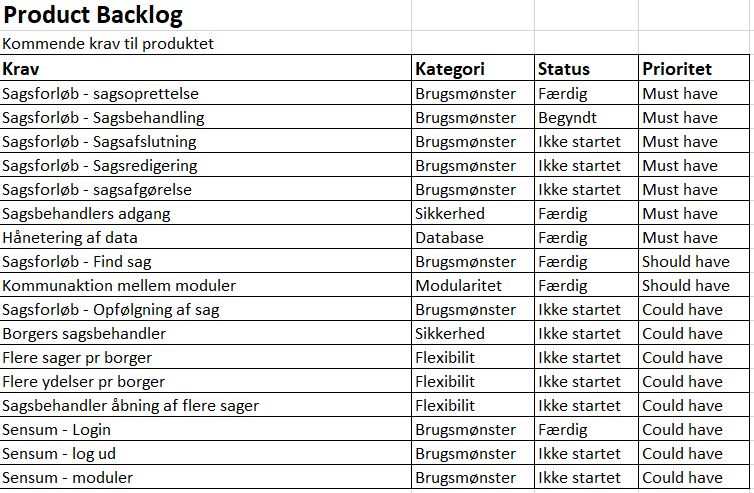
\includegraphics[width = \linewidth]{./PNG/Metoder/product_backlog.png}
  \caption{Gruppens product backlog}
  \label{fig:productbacklog}
\end{figure}
\\Baseret på to iterationer har gruppen valgt at 1. iteration skulle være general funktionalitet og når gruppen nåede 2. iteration, skulle der implementeres GUI og database. 
Planlægningen skete ud fra kanban board, hvor der blev oprettet opgaver som hvert par blev tildelt og herefter blev opgaven udarbejdet. 
Generelt har gruppen ikke fundet Scrum særlig anvendelig i projektet. 
Dette skyldes flere årsager. 
I forhold til rollefordelingen, så har gruppen ikke haft en bestemt product owner for projektet. 
Dette skyldes at gruppen ikke var et fuldendt team, hvilket Scrum kræver. 
Der har hellere ikke været benyttet en scrum master fordi gruppen ikke har erfaring nok til at anvende teorien og generelt har der ikke været behov for det. 
Dermed har gruppen valgt at undlade rollefordeling. 
Ydermere blev der udarbejdet en product backlog, men uden en product owner kunne den ikke blive opdateret løbende. 
Til det formål var det bedre og mere effektivt at anvende kanban metoden til at holde styr på hvad der blev udarbejdet og hvad der manglede. 
Som en del af iterationerne har fokus ligget på de forskellige faser og iterationer, hvor gruppen koncentrerede sig om den generelle funktionalitet i første iteration og GUI og database i anden iteration. Det konkluderes, at gruppen har anvendt for meget tid på at forsøge at implementere Scrum i projektet i forhold til udbyttet og udarbejdelsen af en generel oversigt. Som tidligere nævnt blev der udarbejdet en product backlog men uden en product owner til løbende at opdatere den, har gruppen ikke fundet grund til at opdatere det, da det ville være spild af tid og dermed fjerne fokus fra udarbejdelsen af produktet.
